\documentclass[compress]{beamer}
\usetheme{sthlm}

%-=-=-=-=-=-=-=-=-=-=-=-=-=-=-=-=-=-=-=-=-=-=-=-=
%        LOADING BEAMER PACKAGES
%-=-=-=-=-=-=-=-=-=-=-=-=-=-=-=-=-=-=-=-=-=-=-=-=

\usepackage{
booktabs,
datetime,
dtk-logos,
graphicx,
multicol,
pgfplots,
ragged2e,
tabularx,
tikz,
wasysym,
multirow,
float,
caption,
subcaption
}

\pgfplotsset{compat=1.8}

\usepackage[utf8]{inputenc}
\usepackage[portuguese]{babel}
\usepackage[T1]{fontenc}
\usepackage{newpxtext,newpxmath}
\usepackage{listings}

\lstset{ %
language=[LaTeX]TeX,
basicstyle=\normalsize\ttfamily,
keywordstyle=,
numbers=left,
numberstyle=\tiny\ttfamily,
stepnumber=1,
showspaces=false,
showstringspaces=false,
showtabs=false,
breaklines=true,
frame=tb,
framerule=0.5pt,
tabsize=4,
framexleftmargin=0.5em,
framexrightmargin=0.5em,
xleftmargin=0.5em,
xrightmargin=0.5em
}



%-=-=-=-=-=-=-=-=-=-=-=-=-=-=-=-=-=-=-=-=-=-=-=-=
%        LOADING TIKZ LIBRARIES
%-=-=-=-=-=-=-=-=-=-=-=-=-=-=-=-=-=-=-=-=-=-=-=-=

\usetikzlibrary{
backgrounds,
mindmap
}

%-=-=-=-=-=-=-=-=-=-=-=-=-=-=-=-=-=-=-=-=-=-=-=-=
%        BEAMER OPTIONS
%-=-=-=-=-=-=-=-=-=-=-=-=-=-=-=-=-=-=-=-=-=-=-=-=

\setbeameroption{show notes}

%-=-=-=-=-=-=-=-=-=-=-=-=-=-=-=-=-=-=-=-=-=-=-=-=
%        BEAMER COMMANDS
%-=-=-=-=-=-=-=-=-=-=-=-=-=-=-=-=-=-=-=-=-=-=-=-=


%-=-=-=-=-=-=-=-=-=-=-=-=-=-=-=-=-=-=-=-=-=-=-=-=
%
%	PRESENTATION INFORMATION
%
%-=-=-=-=-=-=-=-=-=-=-=-=-=-=-=-=-=-=-=-=-=-=-=-=

\title{Exclusão mútua}
\subtitle{DCE540 - Computação Paralela e Distribuída}
%\date{\small{\jobname}}
\author{\texttt{Iago Carvalho}}
\institute{\texttt{Departamento de Ciência da Computação}}

\hypersetup{
pdfauthor = {Iago A. Carvalho},      
pdfsubject = {Computação Paralela e Distribuída},
pdfkeywords = {},  
pdfmoddate= {D:\pdfdate},          
pdfcreator = {WriteLaTeX}
}

\begin{document}

\begin{frame}
\titlepage

\end{frame}

%% --------------------------------------------------------

\begin{frame}{Acesso a recursos compartilhados}

Em um sistema distribuído, existe um número de aplicações rodando simultaneamente
\begin{itemize}
    \item Duas ou mais aplicações podem querer acessar um mesmo recurso simultaneamente
\end{itemize}

\vspace{0.5cm}

Este acesso simultâneo (concorrente) pode
\begin{itemize}
    \item corromper o recurso
    \item gerar dados inconsistentes
\end{itemize}

\vspace{0.5cm}

Assim, é necessário criar maneiras de coordenar o acesso a recursos distribuídos

\end{frame}

%% --------------------------------------------------------

\begin{frame}{Problemas de acesso compartilhado}

\textbf{Starvation}: Um processo tenta continuamente acessar a um recurso compartilhado, mas nunca consegue acesso
\begin{itemize}
    \item Muito comum quando processos de alta prioridade estão acessando o recurso
    \item Processo fica bloqueado até que o recurso seja liberado
\end{itemize}

\vspace{0.5cm}

\textbf{Deadlock}: Um processo A necessita de um recurso que está sendo acessado por outro processo B. Ao mesmo tempo, o processo B necessita de um recurso que está sendo acessado pelo processo A.
\begin{itemize}
    \item Ambos os processos permanecem bloqueados
    \item Não é possível desfazer o \textit{deadlock} sem mecanismos específicos
\end{itemize}
\end{frame}

%% --------------------------------------------------------

\begin{frame}{Algoritmos para coordenação de acesso}

O \textit{middleware} pode (e deve!) implementar algum tipo de algoritmo para coordenar o acesso a recursos compartilhados

\vspace{0.5cm}

Existem diversos algoritmos diferentes para realizar esta coordenação

\vspace{0.5cm}

Todos os algoritmos devem garantir que
\begin{itemize}
    \item Não ocorra deadlocks
    \item Não ocorra starvation
    \item Equidade e justiça
    \begin{itemize}
        \item Todo processo deve ter chances claras (e parecidas) para acessar o recurso compartilhado
    \end{itemize}
\end{itemize}
\end{frame}

%% --------------------------------------------------------

\begin{frame}{Algoritmo centralizado}

\vspace{1cm}

\centering 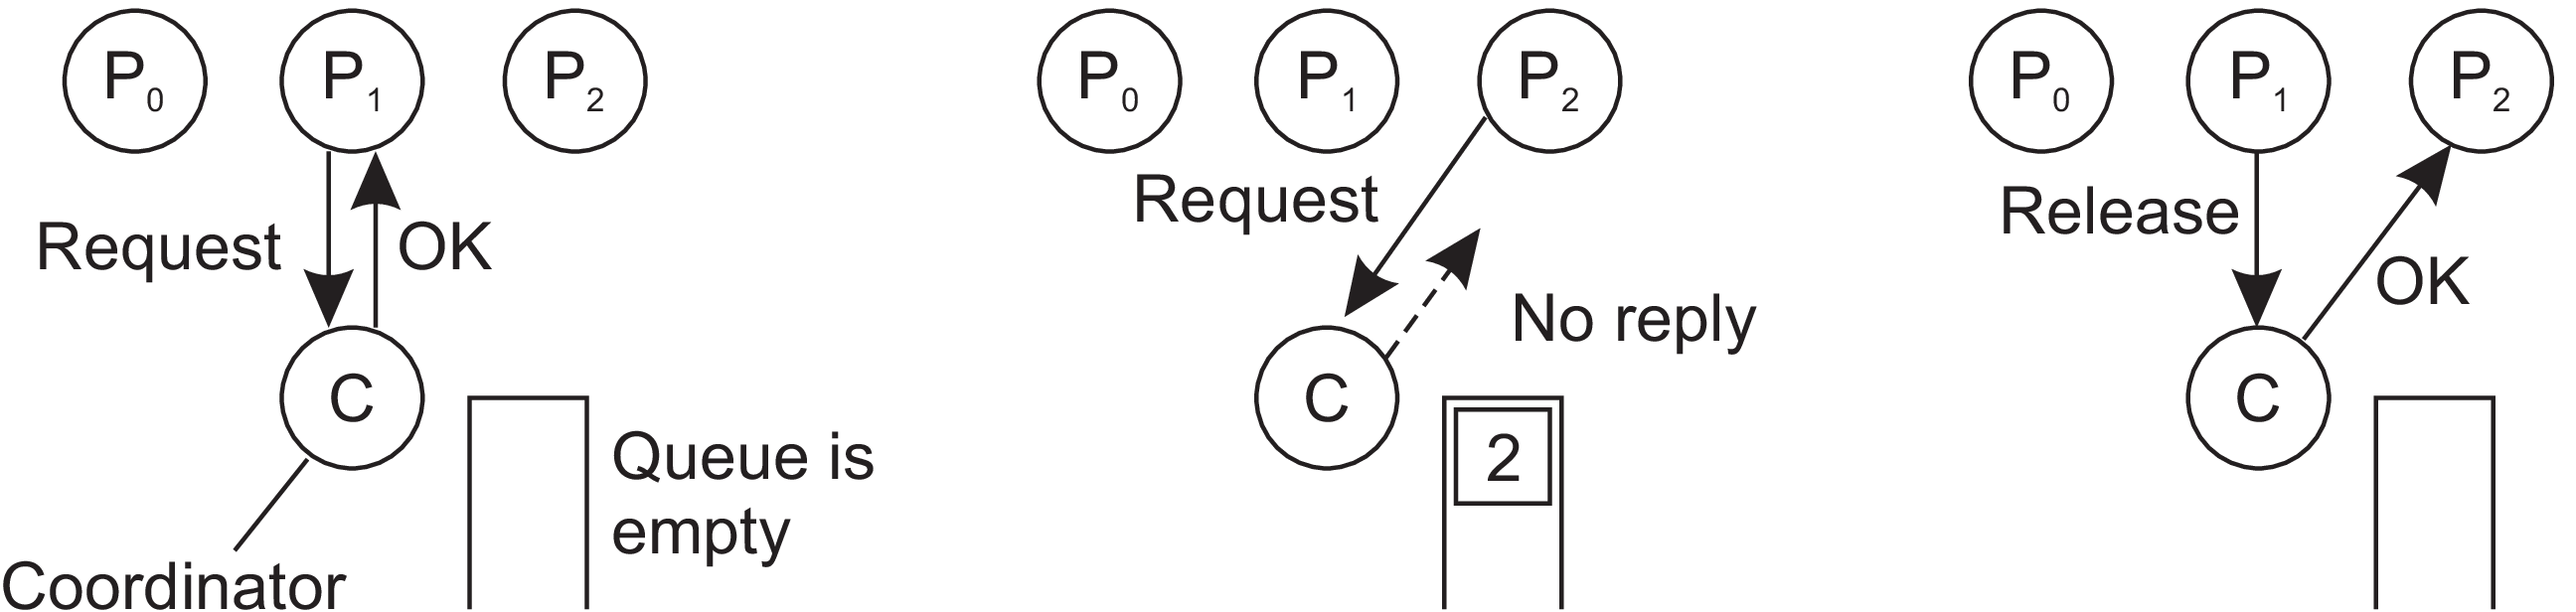
\includegraphics[width=\textwidth]{images/centralizado.png}

\end{frame}

%% --------------------------------------------------------

\begin{frame}{Algoritmo distribuído}

Baseado na ideia de \textit{clocks} lógicos, como discutidos na aula anterior
\begin{itemize}
    \item Baseia-se na ideia de ter uma ordem clara entre todos os eventos no sistema distribuído
    \item Estabelece uma ordem lógica sobre a ordem de acesso aos recursos compartilhados
\end{itemize}

\vspace{0.5cm}

Quando um processo quer acessar um recurso, ele envia uma mensagem para todos os processos do sistema distribuído (includindo ele mesmo)
\begin{itemize}
    \item Nome do recurso compartilhado, número do processo, tempo (lógico)
    \item Assume-se que não existam erros na rede e todos os outros processos leiam a mensagem
\end{itemize}
\end{frame}

%% --------------------------------------------------------

\begin{frame}{Algoritmo distribuído}

Quando um processo recebe uma mensagem de outro, ele pode tomar 3 diferentes ações

\vspace{0.3cm}

Caso ele não esteja acessando o recurso e nem queira acessar
\begin{itemize}
    \item Responde \textit{OK}
\end{itemize}

\vspace{0.3cm}

Caso ele esteja acessando o recurso
\begin{itemize}
    \item Ele enfileira a mensagem e não responde nada
    \item Assim que ele liberar o recurso, ele responde OK
\end{itemize}

\vspace{0.3cm}

Caso ele também queira acessar o recurso
\begin{itemize}
    \item O que possuir a mensagem com a menor data, vence
\end{itemize}

\end{frame}

%% --------------------------------------------------------

\begin{frame}{Algoritmo \textit{token-ring}}

 \vspace{1cm}

\centering 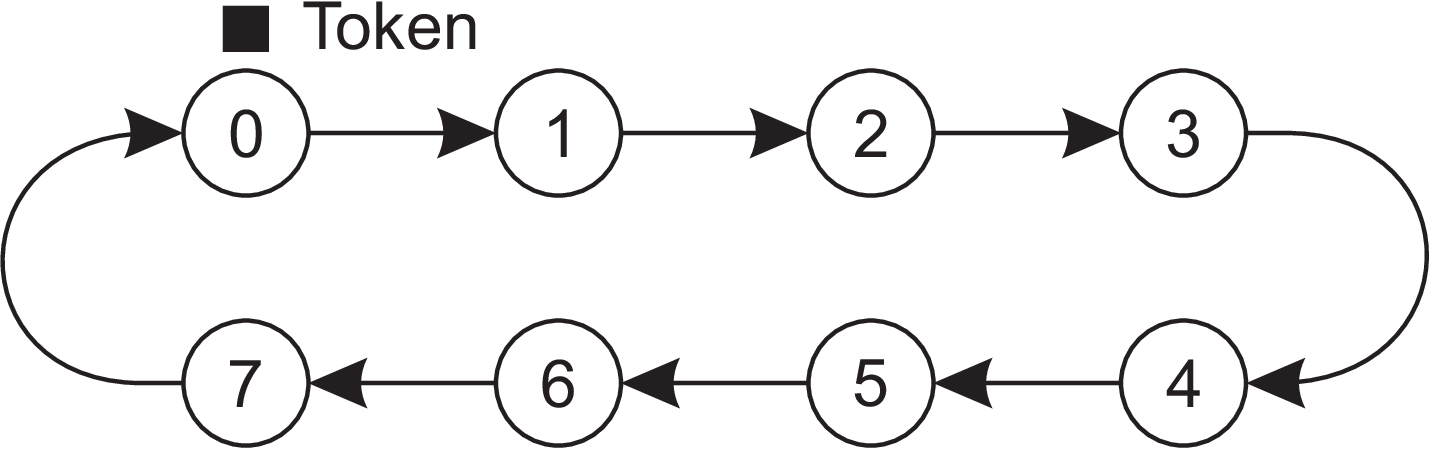
\includegraphics[width=\textwidth]{images/token-ring.png} 
\end{frame}

%% --------------------------------------------------------

\begin{frame}{Comparação entre os algoritmos}

\begin{table}[]
\centering
\begin{tabular}{@{}ccc@{}}
\toprule
Algoritmo    & Mensagens por entrada/saída & Delay      \\ \midrule
Centralizado & $3$                         & $2$          \\
Distribuído  & $3(N - 1)$                  & $2 (N-1)$    \\
Token-ring   & $1, \ldots, \infty$         & $0, \ldots, N-1$ \\ \bottomrule
\end{tabular}%
\end{table}

\end{frame}

\end{document}
